\documentclass[10pt]{article}
\usepackage[margin=2.2cm]{geometry}
\usepackage{booktabs,graphicx,amsmath,xcolor}
% generated by make_report.py -- do not edit
\newcommand{\RAEmerkitDfr}{3.3}
\newcommand{\RAEmerkitEq}{69.8}
\newcommand{\RAEmerkitQviol}{0.2}
\newcommand{\RAEmerkitRed}{0.09}
\newcommand{\RAEmerkitValid}{67.3}
\newcommand{\RAEmerkitXiDfr}{6.5}
\newcommand{\RAEmerkitXiEq}{76.1}
\newcommand{\RAEmerkitXiQviol}{0.2}
\newcommand{\RAEmerkitXiRed}{0.08}
\newcommand{\RAEmerkitXiValid}{71.1}
\newcommand{\RAEmkCpMax}{0.0}
\newcommand{\RAEmkNoIntCpMax}{0.4}
\newcommand{\RAOracleDfr}{0.0}
\newcommand{\RAOracleEq}{78.9}
\newcommand{\RAOracleQviol}{0.2}
\newcommand{\RAOracleRed}{0.07}
\newcommand{\RAOracleValid}{78.7}
\newcommand{\RAOverEmk}{7.8}
\newcommand{\RAOverNoInt}{15.6}
\newcommand{\RAOverRag}{53.8}
\newcommand{\RAOverZeng}{11.8}
\newcommand{\RARagCpMax}{54.7}
\newcommand{\RARagExceed}{99.2}
\newcommand{\RARagMcpDfr}{78.9}
\newcommand{\RARagMcpEq}{100.0}
\newcommand{\RARagMcpPlusFilterDfr}{20.5}
\newcommand{\RARagMcpPlusFilterEq}{100.0}
\newcommand{\RARagMcpPlusFilterQviol}{30.1}
\newcommand{\RARagMcpPlusFilterRed}{1.79}
\newcommand{\RARagMcpPlusFilterValid}{31.3}
\newcommand{\RARagMcpQviol}{55.6}
\newcommand{\RARagMcpRed}{2.25}
\newcommand{\RARagMcpValid}{8.1}
\newcommand{\RAZengDfr}{45.2}
\newcommand{\RAZengEq}{99.5}
\newcommand{\RAZengExceed}{56.8}
\newcommand{\RAZengPlusFilterDfr}{11.5}
\newcommand{\RAZengPlusFilterEq}{82.0}
\newcommand{\RAZengPlusFilterQviol}{0.1}
\newcommand{\RAZengPlusFilterRed}{0.04}
\newcommand{\RAZengPlusFilterValid}{72.6}
\newcommand{\RAZengQviol}{0.6}
\newcommand{\RAZengRed}{0.07}
\newcommand{\RAZengValid}{54.5}
\newcommand{\RBAmbEpsZeroFive}{10.9}
\newcommand{\RBDfrThree}{3.2}
\newcommand{\RBEpsThree}{0.070}
\newcommand{\RBEqEpsZero}{22.7}
\newcommand{\RBEqHigh}{77.9}
\newcommand{\RBEqHundred}{26.1}
\newcommand{\RBEqLow}{26.1}
\newcommand{\RBEqThree}{69.8}
\newcommand{\RBMaxDfrRatio}{0.69}
\newcommand{\RCapPrec}{100.0}
\newcommand{\RCapRec}{96.6}
\newcommand{\RConfCovFive}{95.9}
\newcommand{\RConfCovTen}{92.7}
\newcommand{\RConfCovTwenty}{91.5}
\newcommand{\RDAdditiveUtilityDfr}{4.5}
\newcommand{\RDAdditiveUtilityEq}{69.8}
\newcommand{\RDAdditiveUtilityQviol}{0.0}
\newcommand{\RDAdditiveUtilityRed}{1.10}
\newcommand{\RDDeclaredAnnotationsDfr}{19.0}
\newcommand{\RDDeclaredAnnotationsEq}{80.9}
\newcommand{\RDDeclaredAnnotationsQviol}{0.2}
\newcommand{\RDDeclaredAnnotationsRed}{0.08}
\newcommand{\RDFullEmerkitDfr}{3.3}
\newcommand{\RDFullEmerkitEq}{69.8}
\newcommand{\RDFullEmerkitQviol}{0.2}
\newcommand{\RDFullEmerkitRed}{0.09}
\newcommand{\RDNoInteractionsDfr}{3.3}
\newcommand{\RDNoInteractionsEq}{69.8}
\newcommand{\RDNoInteractionsQviol}{0.2}
\newcommand{\RDNoInteractionsRed}{0.14}
\newcommand{\RDNoQosDfr}{4.1}
\newcommand{\RDNoQosEq}{76.5}
\newcommand{\RDNoQosQviol}{46.1}
\newcommand{\RDNoQosRed}{0.23}
\newcommand{\RLabAccMax}{95.9}
\newcommand{\RLabAccMin}{85.7}
\newcommand{\RNSeeds}{5}
\newcommand{\RNTasks}{1500}

% generated by make_report2.py
\newcommand{\RAfourEmk}{82.2}
\newcommand{\RAfourEmkSevenFive}{11.1}
\newcommand{\RAfourRag}{8.4}
\newcommand{\RAfourZeng}{60.9}
\newcommand{\RAfourZengSevenFive}{10.0}
\newcommand{\RAuAgree}{26}
\newcommand{\RAuLowConf}{5}
\newcommand{\RAuOut}{24}
\newcommand{\RAuReviewed}{40}
\newcommand{\RAuServers}{40}
\newcommand{\RAuTools}{210}
\newcommand{\RBthreeDeclMax}{16.7}
\newcommand{\RBthreeEmkMax}{3.3}
\newcommand{\RBthreeZengHigh}{15.6}
\newcommand{\RBtwoDeclMeight}{18.2}
\newcommand{\RBtwoDeclMzero}{3.4}
\newcommand{\RBtwoEmkMax}{5.7}
\newcommand{\RBtwoEmkMin}{3.3}
\newcommand{\RBtwoEqWtwenty}{67.8}
\newcommand{\RBtwoEqWzero}{87.3}
\newcommand{\RBtwoRagMax}{21.8}
\newcommand{\RBtwoZengMax}{14.8}
\newcommand{\RCfourEmkLarge}{8}
\newcommand{\RCfourEmkSmall}{7}
\newcommand{\RCfourMem}{270}
\newcommand{\RCfourPrep}{1.00}
\newcommand{\RCfourReal}{0.3}
\newcommand{\RCthreeConf}{2.3}
\newcommand{\RCthreeInfFive}{85.9}
\newcommand{\RCthreeMedMax}{0.16}
\newcommand{\RCthreePmax}{0.31}
\newcommand{\RCthreeTo}{0.0}
\newcommand{\RCtwoAllCons}{79.2}
\newcommand{\RCtwoAllThree}{84.7}
\newcommand{\RCtwoAllTwo}{83.3}
\newcommand{\RCtwoAllZero}{55.6}
\newcommand{\RCtwoNoWf}{0.0}
\newcommand{\RCtwoObjMin}{99.3}
\newcommand{\RCtwoPrereq}{0}
\newcommand{\RCtwoPres}{0}
\newcommand{\RCtwoRagRisk}{100.0}
\newcommand{\RCtwoSub}{9.7}
\newcommand{\RCtwoTaskDfr}{6.9}
\newcommand{\RCtwoWfRisk}{34.7}
\newcommand{\RCtwoWfRiskCons}{37.5}
\newcommand{\RCtwoZAll}{93.1}
\newcommand{\RCtwoZRisk}{91.7}
\newcommand{\RCtwoZfAll}{56.9}
\newcommand{\RCtwoZfRisk}{36.1}
\newcommand{\RDtwoRedI}{0.07}
\newcommand{\RDtwoRedNoI}{0.14}
\newcommand{\RDtwoValidMax}{83.6}
\newcommand{\RDtwoValidMin}{82.2}
\newcommand{\REoneRiskStd}{7.1}
\newcommand{\REoneRiskStrict}{11.2}
\newcommand{\REoneSafeSyn}{89.1}
\newcommand{\REoneUncMix}{13.1}
\newcommand{\REoneUncSyn}{3.8}
\newcommand{\REtwoUncHalf}{1.3}
\newcommand{\RFoneBlocked}{100.0}
\newcommand{\RFoneDenied}{2.8}
\newcommand{\RFoneExact}{100.0}
\newcommand{\RFoneExposed}{100.0}
\newcommand{\RFoneN}{72}
\newcommand{\RFoneSec}{1.3}
\newcommand{\RFoneSeeds}{3}

% generated by make_report3.py
\newcommand{\RAfiveAucBase}{0.52}
\newcommand{\RAfiveAucConf}{0.73}
\newcommand{\RAfiveAucSim}{0.82}
\newcommand{\RAfiveCoefConf}{-3.42}
\newcommand{\RAfiveCoefLoad}{0.03}
\newcommand{\RAfiveCoefSat}{0.007}
\newcommand{\RAfiveCoefSim}{-0.91}
\newcommand{\RAfiveHaikuConf}{84.8}
\newcommand{\RAfiveHaikuRand}{99.2}
\newcommand{\RAfiveModels}{2}
\newcommand{\RAfiveN}{1000}
\newcommand{\RAfiveOpusConf}{81.6}
\newcommand{\RAfiveOpusRand}{99.6}
\newcommand{\RAfivePConf}{< 0.001}
\newcommand{\RAfivePLoad}{0.91}
\newcommand{\RAfivePSat}{0.022}
\newcommand{\RAfiveSyn}{98.2}
\newcommand{\RAuHaikuAgree}{19}
\newcommand{\RAuHaikuDec}{168}
\newcommand{\RAuHaikuN}{34}
\newcommand{\RAuPair}{152}
\newcommand{\RAuPairN}{168}
\newcommand{\RAuSonnetAgree}{30}
\newcommand{\RAuSonnetDec}{209}
\newcommand{\RAuSonnetN}{40}
\newcommand{\RCoCpEq}{100.0}
\newcommand{\RCoCpObj}{70.8}
\newcommand{\RCoCpRisk}{100.0}
\newcommand{\RCoLgEq}{84.8}
\newcommand{\RCoLgObj}{100.0}
\newcommand{\RCoLgPrereq}{0}
\newcommand{\RCoLgRaw}{91.7}
\newcommand{\RCoLgRisk}{13.3}
\newcommand{\RCoLgValid}{83.3}
\newcommand{\RCoN}{72}
\newcommand{\RCoSeeds}{3}
\newcommand{\RFlBlocked}{100.0}
\newcommand{\RFlDenied}{0}
\newcommand{\RFlExposed}{100.0}
\newcommand{\RFlN}{27}
\newcommand{\RFlRealised}{22.1}
\newcommand{\RFlSeeds}{3}
\newcommand{\RFlUnexp}{0}
\newcommand{\RJfCorr}{0.67}
\newcommand{\RJfGap}{0.23}
\newcommand{\RJfInter}{0.85}
\newcommand{\RJnAgree}{93.5}
\newcommand{\RJnDis}{7}
\newcommand{\RJnItems}{108}
\newcommand{\RJnKappa}{1.00}
\newcommand{\RJsAgree}{73.7}
\newcommand{\RJsDis}{5}
\newcommand{\RJsItems}{19}
\newcommand{\RJsKappa}{0.91}
\newcommand{\RLaMapRec}{95.9}
\newcommand{\RLaPrec}{100.0}
\newcommand{\RLaRec}{97.1}
\newcommand{\RPonePanelDfr}{2.4}
\newcommand{\RPonePanelEq}{83.6}
\newcommand{\RPonePanelZfDfr}{7.4}
\newcommand{\RPoneStandardDfr}{3.4}
\newcommand{\RPoneStandardEq}{85.3}
\newcommand{\RPoneStandardZfDfr}{4.8}
\newcommand{\RPtwoPanelAll}{81.9}
\newcommand{\RPtwoPanelRisk}{30.6}
\newcommand{\RPtwoPanelSub}{14.1}
\newcommand{\RPtwoStandardAll}{83.3}
\newcommand{\RPtwoStandardRisk}{34.7}
\newcommand{\RPtwoStandardSub}{9.7}
\newcommand{\RSixEmk}{73.8}
\newcommand{\RSixEmkAvail}{77.6}
\newcommand{\RSixEmkClones}{0.68}
\newcommand{\RSixN}{500}
\newcommand{\RSixP}{0.25}
\newcommand{\RSixRag}{73.0}
\newcommand{\RSixRagAvail}{76.6}
\newcommand{\RSixRagClones}{1.67}
\newcommand{\RSixRnd}{42.2}
\newcommand{\RSixRndAvail}{43.6}
\newcommand{\RSixRndClones}{1.08}

\title{EmerKit: experimental results without language models\\\large Final data, with language models (Claude family only) --- \textcolor{red!60!black}{working report}}
\date{}
\begin{document}

\maketitle

\noindent Every number in this document is generated from the result files by \texttt{make\_report.py}; none is typed by hand.

\section{Setup}
The pilot runs on a synthetic catalogue of educational MCP servers with complete ground truth (capabilities, the learner data each tool returns, whether it forwards content beyond its server, receiver roles, confusable pairs), regenerated for each of \RNSeeds{} seeds (about 165 tools on 36 servers per seed). Tasks are generated independently of any scenario from concept graphs in three domains: data science (LectureBank 2.0, human-annotated prerequisites), programming (expert-authored after CS2023) and English as a foreign language (expert-authored after the CEFR): 300 test tasks per seed, 50 per pedagogical type, \RNTasks{} in total. Default parameters: $B=2000$ tokens, $\theta=0.75$, $k_{\max}=4$, $N=20$, $\tau=1.25$, target risk $\xi=0.05$, $\zeta=0.1$, 300 calibration tasks and a level grid refined near zero ($0.001$ to $0.02$, then steps of $0.025$ up to $0.5$); 40\% of annotations are present, 5\% of them are wrong, and observable cues appear in 40\% of the descriptions. No language model is called: capabilities are extracted by a similarity mapper and labels by weak supervision.

A toolkit is \emph{valid} when it is returned, covers every required capability, makes no denied flow possible under the true labels, and meets the QoS bounds of its task. DFR is the share of returned toolkits with at least one denied flow. Baselines are RAG-MCP (top-$k$ by relevance) and the integer program of Zeng et al. (one service per capability, global QoS constraints), each with and without a filter on declared annotations. The \emph{oracle} is EmerKit given the true labels; it bounds what any label-inference method can achieve.

\section{Preparation quality (series A0 and B0)}
Capability extraction reaches a precision of \RCapPrec\% and a recall of \RCapRec\%; synthetic descriptions are easier than real ones, so this figure is optimistic. Label classifiers reach an accuracy between \RLabAccMin\% and \RLabAccMax\% depending on the label. The empirical coverage of the conformal sets is \RConfCovFive\%, \RConfCovTen\%, and \RConfCovTwenty\% for $\epsilon=0.05$, $0.1$, and $0.2$, so it stays at or above the nominal $1-\epsilon$ in all three cases, as split conformal prediction guarantees.

\section{Reference comparison (series A1)}
% generated by make_report.py -- do not edit
\begin{table}[!ht]\centering\caption{Series A1 (pilot): reference comparison on the synthetic catalogue, 1500 tasks over 5 seeds. Rates in \%, with 95\% bootstrap intervals; DFR, QoS violation and redundancy are computed over equipped tasks.}\label{tab:a1}
\scriptsize\begin{tabular}{lrrrrr}\toprule
Method & Equipped & Valid & DFR & QoS viol. & Redund. \\ \midrule
EmerKit & 69.8 [67.4, 72.1] & 67.3 [64.9, 69.7] & 3.3 & 0.2 & 0.09 \\
EmerKit-xi0.10 & 76.1 [73.9, 78.3] & 71.1 [68.8, 73.3] & 6.5 & 0.2 & 0.08 \\
Oracle & 78.9 [76.8, 80.9] & 78.7 [76.6, 80.7] & 0.0 & 0.2 & 0.07 \\
RAG-MCP & 100.0 [100.0, 100.0] & 8.1 [6.7, 9.5] & 78.9 & 55.6 & 2.25 \\
RAG-MCP+filter & 100.0 [100.0, 100.0] & 31.3 [29.0, 33.7] & 20.5 & 30.1 & 1.79 \\
Zeng & 99.5 [99.1, 99.8] & 54.5 [52.1, 57.0] & 45.2 & 0.6 & 0.07 \\
Zeng+filter & 82.0 [80.0, 83.9] & 72.6 [70.3, 74.9] & 11.5 & 0.1 & 0.04 \\
\bottomrule\end{tabular}\end{table}
\begin{table}[!ht]\centering\caption{Series B1 (pilot): calibrated level $\hat\epsilon$ and test denied-flow rate (over equipped tasks) for each target risk $\xi$ and number of calibration tasks, $\zeta=0.1$; means over seeds.}\label{tab:b1}
\scriptsize\begin{tabular}{rrrrr}\toprule $\xi$ & $n_{cal}$ & $\hat\epsilon$ & DFR (\%) & Equipped (\%) \\ \midrule
0.05 & 45 & 0.025 & 0.7 & 38.1 \\
0.05 & 100 & 0.018 & 0.3 & 26.1 \\
0.05 & 200 & 0.037 & 1.8 & 46.3 \\
0.05 & 300 & 0.070 & 3.2 & 69.8 \\
0.10 & 45 & 0.133 & 3.3 & 57.7 \\
0.10 & 100 & 0.090 & 4.9 & 75.5 \\
0.10 & 200 & 0.335 & 6.9 & 76.1 \\
0.10 & 300 & 0.335 & 6.9 & 76.1 \\
0.20 & 45 & 0.500 & 9.6 & 77.9 \\
0.20 & 100 & 0.500 & 9.6 & 77.9 \\
0.20 & 200 & 0.500 & 9.6 & 77.9 \\
0.20 & 300 & 0.500 & 9.6 & 77.9 \\
\bottomrule\end{tabular}\end{table}
\begin{table}[!ht]\centering\caption{Sample-size rule of the task-level calibration: largest number of violations among $n_{cal}$ audited calibration tasks that still certifies a level, for $\zeta=0.1$ (computed from the binomial distribution).}\label{tab:power}
\scriptsize\begin{tabular}{lrrrrr}\toprule $n_{cal}$ & 45 & 100 & 200 & 300 & 500 \\ \midrule
$\xi=0.05$ & 0 & 1 & 5 & 9 & 18 \\
$\xi=0.10$ & 1 & 5 & 14 & 22 & 40 \\
\bottomrule\end{tabular}\end{table}
\begin{table}[!ht]\centering\caption{Series D1 (pilot): ablations at the calibrated level. Rates in \%; DFR, QoS violation and redundancy over equipped tasks.}\label{tab:d1}
\scriptsize\begin{tabular}{lrrrrr}\toprule Variant & Equipped & Valid & DFR & QoS viol. & Redund. \\ \midrule
full EmerKit & 69.8 & 67.3 & 3.3 & 0.2 & 0.09 \\
additive utility & 69.8 & 66.7 & 4.5 & 0.0 & 1.10 \\
no interactions & 69.8 & 67.3 & 3.3 & 0.2 & 0.14 \\
no QoS & 76.5 & 39.9 & 4.1 & 46.1 & 0.23 \\
declared annotations & 80.9 & 65.4 & 19.0 & 0.2 & 0.08 \\
\bottomrule\end{tabular}\end{table}


\begin{figure}[t]\centering
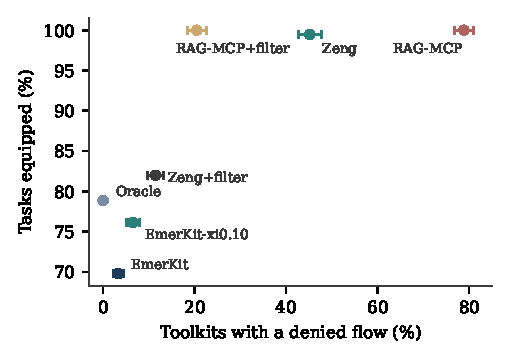
\includegraphics[width=0.48\linewidth]{fig_a1_tradeoff.pdf}\hfill
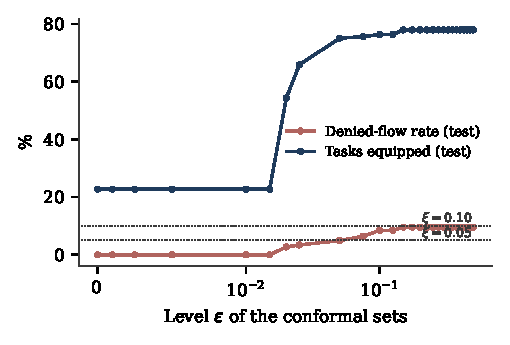
\includegraphics[width=0.48\linewidth]{fig_b1_calibration.pdf}
\caption{Left: tasks equipped against the denied-flow rate of returned toolkits (series A1; bars are 95\% bootstrap intervals). Right: calibration curve of series B1, averaged over seeds.}\label{fig:a1b1}
\end{figure}

\paragraph{Observations.} Table~\ref{tab:a1} and Fig.~\ref{fig:a1b1} (left) show that EmerKit returns toolkits with a denied flow in \RAEmerkitDfr\% of the equipped tasks, against \RARagMcpDfr\% for RAG-MCP, \RAZengDfr\% for Zeng et al., and still \RARagMcpPlusFilterDfr\% and \RAZengPlusFilterDfr\% when both are filtered on declared annotations. Its toolkits violate the QoS bounds in \RAEmerkitQviol\% of the cases, against \RARagMcpQviol\% for RAG-MCP, and carry almost no redundant provider (\RAEmerkitRed{} per task, against \RARagMcpRed{} for RAG-MCP). In exchange, EmerKit equips \RAEmerkitEq\% of the tasks, against \RAOracleEq\% for the oracle and \RAZengPlusFilterEq\% for Zeng et al. with filter. On the composite criterion, EmerKit produces a valid toolkit for \RAEmerkitValid\% of the tasks, more than RAG-MCP (\RARagMcpValid\%) and Zeng et al. without filter (\RAZengValid\%), but fewer than Zeng et al. with filter (\RAZengPlusFilterValid\%) and the oracle (\RAOracleValid\%). Calibrated at $\xi=0.10$, EmerKit equips \RAEmerkitXiEq\% of the tasks and produces \RAEmerkitXiValid\% valid toolkits, with \RAEmerkitXiDfr\% denied flows.

\paragraph{Interpretation.} The safety result is the expected one: relevance-based selection is blind to flows, QoS-optimal selection is blind to them as well, and a filter on declared annotations cannot see what is not declared. The coverage result is the cost of the guarantee: uncertain tools are excluded in the worst case, and some tasks lose all their admissible toolkits; the gap to the oracle measures this conservatism. Against the filtered QoS baseline, EmerKit trades a few points of valid toolkits for a denied-flow rate several times lower; the paper must state this trade-off as such. Task substitution (series C2) recovers part of the gap.

\section{Calibration (series B1)}
\paragraph{Observations.} In all twelve configurations of Table~\ref{tab:b1}, the test denied-flow rate stays below the target $\xi$; the largest ratio between the two is \RBMaxDfrRatio. At $\xi=0.05$, the share of equipped tasks grows from \RBEqHundred\% with 100 calibration tasks to \RBEqThree\% with 300, for a calibrated level of \RBEpsThree{} and a test denied-flow rate of \RBDfrThree\%. Without label inference ($\epsilon=0$, every set equal to $\{0,1\}$), only \RBEqEpsZero\% of the tasks are equipped (Fig.~\ref{fig:a1b1}, right).
\paragraph{Interpretation.} The task-level calibration delivers what Proposition~3 states on held-out tasks: the risk bound holds for the toolkits that the composer actually returns. Its usefulness depends on statistical power. With few calibration tasks, the test tolerates almost no violation (Table~\ref{tab:power}): at $\xi=0.05$, 100 tasks tolerate a single one, so the fixed-sequence test stops at a very conservative level even when the true risk is well below the target. With 300 tasks and a grid refined near zero, the test certifies levels at which conformal label inference triples the share of equipped tasks over the purely worst-case check. The paper should state this sample-size rule; for real tools, each calibration task requires the audit of its returned toolkit.

\section{Ablations (series D1)}
\paragraph{Observations.} Replacing the conformal sets by declared annotations raises the share of equipped tasks to \RDDeclaredAnnotationsEq\% but the denied-flow rate to \RDDeclaredAnnotationsDfr\%. Additive utility multiplies the number of redundant providers from \RDFullEmerkitRed{} to \RDAdditiveUtilityRed{} per task. Without QoS, \RDNoQosQviol\% of the toolkits violate their bounds. Removing the interaction terms leaves the equipped share and the denied-flow rate unchanged and raises redundancy from \RDFullEmerkitRed{} to \RDNoInteractionsRed{} redundant providers per task.

\paragraph{Interpretation.} The prediction sets and the worst-case check carry the safety of the approach, and counting each capability once carries most of its parsimony. At the default parameters, interference and saturation have little to act on: near-duplicates are rare and toolkits use a small part of the budget. Their effect is examined under stress in the next section.

\section{Interference and context load (series A2 and A3)}
\begin{figure}[t]\centering
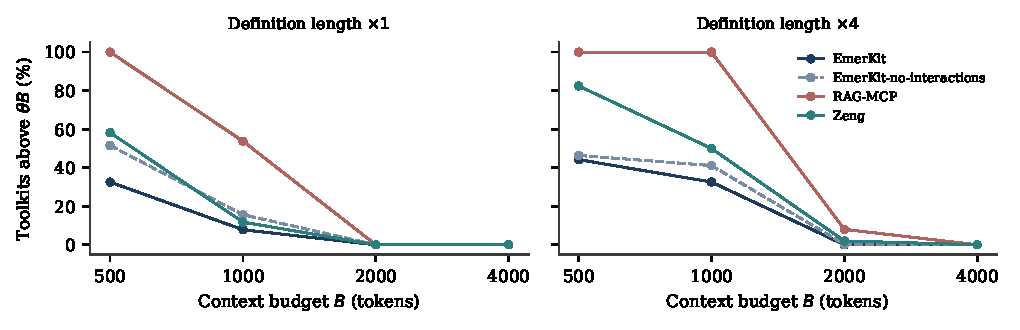
\includegraphics[width=0.9\linewidth]{fig_a3_context.pdf}
\caption{Series A3: share of toolkits whose load exceeds the soft threshold $\theta B$, as a function of the context budget.}\label{fig:a3}
\end{figure}
\paragraph{Observations.} When up to 40\% of the capabilities have a near-duplicate provider, RAG-MCP returns a confusable pair in up to \RARagCpMax\% of its toolkits; EmerKit never does (\RAEmkCpMax\%), and its variant without interaction terms does in at most \RAEmkNoIntCpMax\%. Under a budget of 1{,}000 tokens, \RAOverEmk\% of EmerKit toolkits exceed the soft threshold, against \RAOverNoInt\% without the saturation term, \RAOverZeng\% for Zeng et al., and \RAOverRag\% for RAG-MCP (Fig.~\ref{fig:a3}); at 500 tokens, RAG-MCP exceeds the budget itself in \RARagExceed\% of the cases and Zeng et al. in \RAZengExceed\%.

\paragraph{Interpretation.} On the composition side, avoiding confusable pairs follows mostly from counting each capability once; the interference term removes the residual cases. The saturation term has a clear but moderate effect on context load. Neither result tests the central claim of H1, which concerns the behaviour of an agent: whether these toolkits make an agent choose the right tool more often is the object of the selection probes (series A5 and A6), which require model calls.

\section{QoS bounds (series A4)}
\paragraph{Observations.} Grid series use a fixed level $\epsilon=0.05$ and three seeds (Table~\ref{tab:a4}). With bounds set at $1.25$ times the median aggregate, EmerKit returns a valid toolkit for \RAfourEmk\% of the tasks, against \RAfourZeng\% for Zeng et al. and \RAfourRag\% for RAG-MCP. When the bounds tighten to $0.75$, the shares fall to \RAfourEmkSevenFive\% and \RAfourZengSevenFive\%; at $0.5$ no method returns a valid toolkit.
\paragraph{Interpretation.} QoS and flow constraints combine: Zeng et al. meet the bounds but not the norms, RAG-MCP meets neither. The share of valid toolkits depends strongly on how bounds are set, which the paper must state when it reports a single value.

\section{Imperfect metadata (series B2)}
\paragraph{Observations.} Across all ten configurations of Table~\ref{tab:b2}, the denied-flow rate of EmerKit stays between \RBtwoEmkMin\% and \RBtwoEmkMax\%. With declared annotations instead of prediction sets, it rises from \RBtwoDeclMzero\% when every annotation is present to \RBtwoDeclMeight\% when 80\% are missing; filtered baselines reach up to \RBtwoRagMax\% (RAG-MCP) and \RBtwoZengMax\% (Zeng et al.). The price is coverage: when the share of wrong annotations grows from 0 to 20\%, EmerKit equips \RBtwoEqWzero\% then \RBtwoEqWtwenty\% of the tasks.
\paragraph{Interpretation.} This is the main evidence for H2: the risk of EmerKit does not depend on how many annotations providers publish, whereas every method that trusts declarations degrades with them. Wrong annotations do not raise its risk; they widen the prediction sets and make it more conservative.

\section{Norms and receivers (series B3)}
\paragraph{Observations.} Under the three norm profiles and three shares of third-party providers (Table~\ref{tab:b3}), the denied-flow rate of EmerKit never exceeds \RBthreeEmkMax\%. That of Zeng et al. with filter reaches \RBthreeZengHigh\% when third-party providers dominate, and that of EmerKit with declared annotations \RBthreeDeclMax\%.
\paragraph{Interpretation.} The flow check adapts to the norm base as intended; the filtered QoS baseline is safe only as long as few providers are third parties.

\section{Sensitivity to the weights (series D2)}
\paragraph{Observations.} Over eleven settings of $\lambda_I$, $\lambda_C$, $\lambda_Q$ and $\theta$ (Table~\ref{tab:d2}), the share of valid toolkits stays between \RDtwoValidMin\% and \RDtwoValidMax\%. The interference weight changes redundancy only: \RDtwoRedNoI{} redundant providers per task without it, \RDtwoRedI{} with it.
\paragraph{Interpretation.} The composer is not sensitive to its provisional weights at default load and confusability, so the comparisons above do not hinge on tuning. The weights matter where interactions are frequent (series A2, A3), and their values must come from the selection probes.

\section{End-to-end composition and substitution (series C2, and C1 without language models)}
\paragraph{Observations.} The generator produced no valid workflow for \RCtwoNoWf\% of the requests; these requests are excluded for every method in Table~\ref{tab:c2}. Without substitution, every task of the workflow is equipped for \RCtwoAllZero\% of the requests; with at most two substitutions, for \RCtwoAllTwo\% (\RCtwoAllThree\% with three), and \RCtwoSub\% of the tasks are substituted. The same generator followed by Zeng et al. with filter equips every task for \RCtwoZfAll\% of the requests. The final workflows cover at least \RCtwoObjMin\% of the target concepts, with \RCtwoPrereq{} prerequisite violations and \RCtwoPres{} substitution outside the preservation relation over all configurations. Per task, \RCtwoTaskDfr\% of EmerKit toolkits make a denied flow possible, so that \RCtwoWfRisk\% of the workflows contain at least one such toolkit, against \RCtwoZfRisk\% with Zeng et al. with filter, \RCtwoZRisk\% without filter, and \RCtwoRagRisk\% with RAG-MCP. In conservative mode, these figures are \RCtwoWfRiskCons\% and \RCtwoAllCons\%.
\paragraph{Interpretation.} Substitution delivers what it is designed for: it turns a large share of incomplete workflows into complete ones without leaving the substitution catalogue. Two findings call for changes. First, the guarantee is stated per task, and risk accumulates over the tasks of a workflow; bounding the risk of a whole workflow requires calibrating each task at $\xi/|V|$, or calibrating on whole workflows. Second, at a fixed level the per-task rate exceeds the target of 5\%: end-to-end tasks inherit attributes through hand-offs and differ from the calibration distribution, which is exactly the shift the guarantee does not cover. Both points must be stated in the paper.

\section{Solver and catalogue scaling (series C3 and C4)}
\paragraph{Observations.} The median solving time per task never exceeds \RCthreeMedMax{} s and the 95th percentile \RCthreePmax{} s, with no time-out in any configuration (Table~\ref{tab:c3}); with five required capabilities, \RCthreeInfFive\% of the tasks have no admissible toolkit, and the minimal conflict contains \RCthreeConf{} constraint groups on average. With up to 2{,}960 tools drawn from MCP-tools and the Toucan server catalogue (Table~\ref{tab:c4}), preparation takes \RCfourPrep{} s, the median time per task moves from \RCfourEmkSmall{} to \RCfourEmkLarge{} ms, memory stays below \RCfourMem{} MB, and at most \RCfourReal\% of the toolkits use a real server.
\paragraph{Interpretation.} Exact composition is practical at the sizes considered, and the cost of the approach is in preparation, not in composition. Real tools are rarely selected because few of them provide educational capabilities and none is annotated, so their labels stay uncertain.

\section{Gap map (series E1 and E2)}
\paragraph{Observations.} On the synthetic catalogue with standard norms, \REoneSafeSyn\% of the demand-weighted archetypes are safe, \REoneUncSyn\% uncertain and \REoneRiskStd\% risky (Table~\ref{tab:e1}); strict norms raise the risky share to \REoneRiskStrict\%, and adding MCP-tools raises the uncertain share to \REoneUncMix\%. When providers annotate half of the tools correctly, the uncertain share falls to \REtwoUncHalf\% (Table~\ref{tab:e2}).
\paragraph{Interpretation.} The classes react to the levers they are meant to expose: norms create risky archetypes, undocumented tools create uncertain ones, and publishing annotations resolves them. No archetype is uncovered because the synthetic catalogue provides every capability; the uncovered class can only be tested on real catalogues.

% generated by make_report2.py
\begin{table}[!ht]\centering\caption{Series A4: share of valid toolkits (\%) as a function of the tightness $\tau$ of the QoS bounds.}\label{tab:a4}\scriptsize
\begin{tabular}{lrrr}\toprule
tau & EmerKit & RAG-MCP & Zeng \\ \midrule
0.5 & 0.0 & 0.0 & 0.0 \\
0.75 & 11.1 & 0.0 & 10.0 \\
1.0 & 71.8 & 6.2 & 55.6 \\
1.25 & 82.2 & 8.4 & 60.9 \\
1.5 & 83.8 & 8.7 & 60.0 \\
\bottomrule\end{tabular}\end{table}
\begin{table}[!ht]\centering\caption{Series B2: denied-flow rate over equipped tasks and share of equipped tasks (\%) under missing ($m$) and wrong ($w$) annotations and cue strength; level fixed at $\epsilon=0.05$.}\label{tab:b2}\scriptsize
\begin{tabular}{lllrrrrrrr}\toprule
m & w & cue & EmerKit & EmerKit-declared & RAG-MCP+filter & Zeng+filter & EmerKit (eq.) & Oracle (eq.) & Zeng+filter (eq.) \\ \midrule
0.0 & 0.05 & 0.4 & 3.4 & 3.4 & 2.9 & 1.0 & 91.8 & 90.9 & 91.6 \\
0.2 & 0.05 & 0.4 & 3.9 & 13.4 & 15.6 & 1.7 & 91.6 & 90.9 & 91.8 \\
0.4 & 0.05 & 0.4 & 3.3 & 16.4 & 17.3 & 3.4 & 88.0 & 90.9 & 92.4 \\
0.6 & 0.0 & 0.4 & 3.3 & 18.1 & 18.4 & 5.2 & 87.3 & 90.9 & 94.0 \\
0.6 & 0.05 & 0.2 & 4.8 & 14.0 & 17.1 & 14.8 & 74.4 & 82.4 & 87.1 \\
0.6 & 0.05 & 0.4 & 3.4 & 18.2 & 18.7 & 4.8 & 85.3 & 90.9 & 93.3 \\
0.6 & 0.05 & 0.6 & 5.7 & 15.5 & 15.8 & 10.2 & 78.0 & 87.1 & 91.1 \\
0.6 & 0.1 & 0.4 & 3.7 & 17.8 & 21.6 & 7.1 & 71.8 & 90.9 & 93.3 \\
0.6 & 0.2 & 0.4 & 3.6 & 16.8 & 21.8 & 8.4 & 67.8 & 90.9 & 86.9 \\
0.8 & 0.05 & 0.4 & 4.5 & 18.2 & 20.0 & 9.4 & 79.8 & 90.9 & 94.7 \\
\bottomrule\end{tabular}\end{table}
\begin{table}[!ht]\centering\caption{Series B3: denied-flow rate over equipped tasks (\%) by norm profile and share of third-party providers (bias).}\label{tab:b3}\scriptsize
\begin{tabular}{llrrrr}\toprule
profile & ext bias & EmerKit & EmerKit-declared & RAG-MCP+filter & Zeng+filter \\ \midrule
permissive & 0.5 & 1.1 & 8.3 & 15.7 & 2.1 \\
permissive & 1.0 & 2.1 & 12.1 & 16.2 & 5.5 \\
permissive & 2.0 & 0.6 & 11.4 & 14.4 & 12.9 \\
standard & 0.5 & 1.2 & 10.4 & 20.4 & 5.2 \\
standard & 1.0 & 3.3 & 16.7 & 18.5 & 2.6 \\
standard & 2.0 & 0.0 & 10.1 & 14.4 & 11.1 \\
strict & 0.5 & 0.6 & 12.1 & 22.2 & 5.0 \\
strict & 1.0 & 1.2 & 16.0 & 22.7 & 2.2 \\
strict & 2.0 & 0.0 & 15.9 & 19.4 & 15.6 \\
\bottomrule\end{tabular}\end{table}
\begin{table}[!ht]\centering\caption{Series D2: sensitivity of EmerKit to its weights (one factor at a time; rates in \%, redundancy per task).}\label{tab:d2}\scriptsize
\begin{tabular}{llllrrrrr}\toprule
lam I & lam C & lam Q & theta & eq & valid & dfr e & red e & over e \\ \midrule
0.0 & 1.0 & 0.5 & 0.75 & 85.3 & 82.2 & 3.4 & 14.3 & 0.0 \\
0.5 & 1.0 & 0.5 & 0.75 & 85.3 & 82.2 & 3.4 & 8.3 & 0.0 \\
1.0 & 0.0 & 0.5 & 0.75 & 85.3 & 82.2 & 3.4 & 7.0 & 0.0 \\
1.0 & 0.5 & 0.5 & 0.75 & 85.3 & 82.2 & 3.4 & 7.0 & 0.0 \\
1.0 & 1.0 & 0.0 & 0.75 & 85.3 & 82.4 & 3.1 & 6.2 & 0.0 \\
1.0 & 1.0 & 0.5 & 0.5 & 85.3 & 82.2 & 3.4 & 6.0 & 0.3 \\
1.0 & 1.0 & 0.5 & 0.75 & 85.3 & 82.2 & 3.4 & 7.0 & 0.0 \\
1.0 & 1.0 & 0.5 & 0.9 & 85.3 & 82.2 & 3.4 & 7.0 & 0.0 \\
1.0 & 1.0 & 1.0 & 0.75 & 85.3 & 83.6 & 1.6 & 7.6 & 0.0 \\
1.0 & 2.0 & 0.5 & 0.75 & 85.3 & 82.2 & 3.4 & 7.0 & 0.0 \\
2.0 & 1.0 & 0.5 & 0.75 & 85.3 & 82.2 & 3.4 & 6.2 & 0.0 \\
\bottomrule\end{tabular}\end{table}
\begin{table}[!ht]\centering\caption{Series C2 and C1 (without language models): end-to-end results per request (\%). Baselines use the same generator, without substitution.}\label{tab:c2}\scriptsize
\begin{tabular}{lllllrrrrrr}\toprule
s max & density & nu & mode & method & equipped & substituted & all equipped & task DFR & workflow risk & objectives \\ \midrule
2 & medium & 0.5 & isolated & EmerKit & 97.8 & 9.7 & 83.3 & 6.9 & 34.7 & 100.0 \\
2 & medium & 0.5 & isolated & Gen+RAG-MCP & 28.4 & 0.0 & 0.0 & 70.8 & 100.0 & 100.0 \\
2 & medium & 0.5 & isolated & Gen+RAG-MCP+filter & 46.1 & 0.0 & 0.0 & 21.4 & 76.4 & 100.0 \\
2 & medium & 0.5 & isolated & Gen+Zeng & 98.8 & 0.0 & 93.1 & 44.0 & 91.7 & 100.0 \\
2 & medium & 0.5 & isolated & Gen+Zeng+filter & 90.2 & 0.0 & 56.9 & 8.6 & 36.1 & 100.0 \\
0 & medium & 0.5 & isolated & EmerKit & 92.3 & 0.0 & 55.6 & 7.4 & 34.7 & 99.3 \\
1 & medium & 0.5 & isolated & EmerKit & 96.6 & 6.4 & 76.4 & 7.4 & 36.1 & 99.3 \\
3 & medium & 0.5 & isolated & EmerKit & 98.0 & 11.9 & 84.7 & 7.4 & 37.5 & 100.0 \\
2 & low & 0.5 & isolated & EmerKit & 97.2 & 9.8 & 79.2 & 7.4 & 37.5 & 100.0 \\
2 & high & 0.5 & isolated & EmerKit & 98.0 & 11.0 & 84.7 & 7.8 & 36.1 & 100.0 \\
2 & medium & 0.1 & isolated & EmerKit & 97.5 & 11.6 & 80.6 & 6.7 & 33.3 & 100.0 \\
2 & medium & 1.0 & isolated & EmerKit & 97.8 & 8.1 & 83.3 & 7.0 & 36.1 & 100.0 \\
2 & medium & 0.5 & conservative & EmerKit & 97.3 & 12.1 & 79.2 & 6.3 & 37.5 & 100.0 \\
\bottomrule\end{tabular}\end{table}
\begin{table}[!ht]\centering\caption{Series C3: solver time per task (s), timeouts and infeasible tasks (\%), and size of the minimal conflict (constraint groups).}\label{tab:c3}\scriptsize
\begin{tabular}{llllrrrrr}\toprule
N & nR & k max & T max & median s & p95 s & timeouts & infeasible & conflict groups \\ \midrule
10 & 3 & 4 & 10.0 & 0.007 & 0.011 & 0.000 & 0.515 & 2.388 \\
20 & 1 & 4 & 10.0 & 0.014 & 0.024 & 0.000 & 0.270 & 1.370 \\
20 & 2 & 4 & 10.0 & 0.020 & 0.142 & 0.000 & 0.233 & 1.571 \\
20 & 3 & 3 & 10.0 & 0.111 & 0.224 & 0.000 & 0.285 & 2.065 \\
20 & 3 & 4 & 1.0 & 0.111 & 0.226 & 0.000 & 0.278 & 1.933 \\
20 & 3 & 4 & 10.0 & 0.111 & 0.225 & 0.000 & 0.278 & 1.933 \\
20 & 3 & 4 & 60.0 & 0.111 & 0.223 & 0.000 & 0.278 & 1.933 \\
20 & 3 & 6 & 10.0 & 0.112 & 0.222 & 0.000 & 0.278 & 1.933 \\
20 & 3 & 8 & 10.0 & 0.111 & 0.223 & 0.000 & 0.278 & 1.933 \\
20 & 5 & 4 & 10.0 & 0.018 & 0.124 & 0.000 & 0.859 & 3.884 \\
30 & 3 & 4 & 10.0 & 0.134 & 0.280 & 0.000 & 0.200 & 1.759 \\
50 & 3 & 4 & 10.0 & 0.158 & 0.313 & 0.000 & 0.100 & 1.407 \\
100 & 3 & 4 & 10.0 & 0.156 & 0.310 & 0.000 & 0.100 & 1.407 \\
\bottomrule\end{tabular}\end{table}
\begin{table}[!ht]\centering\caption{Series C4: preparation time, median time per task (s), memory, and share of toolkits that include a real MCP-tools server.}\label{tab:c4}\scriptsize
\begin{tabular}{lrrrrrrr}\toprule
size & tools & prep s & emerkit med s & rag med s & zeng med s & memory MB & real tools used \\ \midrule
300 & 300 & 0.0994 & 0.0065 & 0.0009 & 0.0019 & 240 & 0.0000 \\
1000 & 1000 & 0.3550 & 0.0067 & 0.0015 & 0.0023 & 245 & 0.0000 \\
2000 & 2000 & 0.6800 & 0.0072 & 0.0020 & 0.0025 & 256 & 0.0000 \\
2960 & 2960 & 0.9964 & 0.0084 & 0.0030 & 0.0028 & 270 & 0.0035 \\
\bottomrule\end{tabular}\end{table}
\begin{table}[!ht]\centering\caption{Series E1: demand-weighted share of task archetypes in each class of the gap map (\%).}\label{tab:e1}\scriptsize
\begin{tabular}{llrrr}\toprule
catalogue & profile & RISKY & SAFE & UNCERTAIN \\ \midrule
mixed & permissive & 5.5 & 84.7 & 9.8 \\
mixed & standard & 7.0 & 79.9 & 13.1 \\
mixed & strict & 11.1 & 71.5 & 17.3 \\
synthetic & permissive & 5.5 & 92.4 & 2.1 \\
synthetic & standard & 7.1 & 89.1 & 3.8 \\
synthetic & strict & 11.2 & 83.3 & 5.5 \\
\bottomrule\end{tabular}\end{table}
\begin{table}[!ht]\centering\caption{Series E2: demand-weighted share of task archetypes in each class of the gap map (\%).}\label{tab:e2}\scriptsize
\begin{tabular}{llrrr}\toprule
remove & annotate & RISKY & SAFE & UNCERTAIN \\ \midrule
0.0 & 0.25 & 7.1 & 89.2 & 3.7 \\
0.0 & 0.5 & 7.5 & 91.2 & 1.3 \\
0.1 & 0.0 & 8.5 & 84.5 & 6.9 \\
0.2 & 0.0 & 18.9 & 78.0 & 3.0 \\
0.3 & 0.0 & 10.4 & 85.9 & 3.7 \\
\bottomrule\end{tabular}\end{table}


\section{Live enactment through the MCP gateway (series F1)}
\paragraph{Observations.} Every server of the synthetic catalogue runs as a real MCP server (official Python SDK) that behaves as its ground truth says: it returns learner data marked by unique canary values and really sends what it receives to the sink of each receiver it reaches. For \RFoneN{} toolkits over \RFoneSeeds{} seeds, the gateway exposed only the tools of the toolkit in \RFoneExposed\% of the runs and refused every call outside it in \RFoneBlocked\%. An exhaustive policy, which calls every tool with everything its parameters can carry, realised exactly the flows predicted by the flow model in \RFoneExact\% of the toolkits; \RFoneDenied\% of the toolkits allowed at least one denied flow, which is the empirical counterpart of the denied-flow rate. A run takes \RFoneSec{} s per task.
\paragraph{Interpretation.} The flow model of Sect.~4.5 is not an approximation of what the runtime does: on these servers, the flows it predicts are the flows that occur. What an LLM agent actually does with the same toolkits (policy \texttt{llm}) requires model calls.

\section{Audit of real tools}
\paragraph{Observations.} Static analysis retrieved the code of \RAuServers{} real servers from GitHub and gathered evidence for \RAuTools{} tools. A model review (Claude) labelled \RAuReviewed{} of them: \RAuOut{} forward what they receive beyond their server, none returns learner data, and \RAuLowConf{} labels have low or medium confidence. The static heuristic agrees with the review on \RAuAgree{} of the \RAuReviewed{} tools.
\paragraph{Interpretation.} Static evidence alone is not an audit: it misses calls made through libraries and over-generalises server-level evidence to every tool. The review is a model judgement and must be declared as such; a human check of a sample remains to be done.

\section{Series with language models}
All model calls below use Claude models (Haiku 5.5, Sonnet 5.5, Opus 5.5); no model of another family was available in this environment, which must be stated as a limitation. Every call is logged.

\paragraph{Capability extraction (A0).} An LLM extractor (Haiku) reaches a precision of \RLaPrec\% and a recall of \RLaRec\% on the synthetic catalogue, against a recall of \RLaMapRec\% for the similarity mapper.

\paragraph{Expert panel.} Three models rated every cell of the norm base, every substitution pair and every cell of the fit matrix. On the \RJnItems{} norm cells they agree unanimously (Fleiss' $\kappa=\RJnKappa$), and their majority matches the norm base on \RJnAgree\% of the cells (\RJnDis{} disagreements: stricter on profile and content sent to third parties during acquisition, more permissive for contracted processors in assessment). On the \RJsItems{} substitution pairs rated by all three ($\kappa=\RJsKappa$), the majority matches the catalogue on \RJsAgree\% of the pairs; the models reject the acquisition--discussion and practice--production substitutions. Their fit ratings correlate at \RJfCorr{} with the matrix (\RJfInter{} between models; mean gap \RJfGap). These are model judgements, not a validation by instructors.

\paragraph{Sensitivity to the panel (P1, P2).} With the panel's majority norms at the task level, EmerKit equips \RPonePanelEq\% of the tasks (\RPoneStandardEq\% with the standard base) with a denied-flow rate of \RPonePanelDfr\% (\RPoneStandardDfr\%), and Zeng et al. with filter reaches \RPonePanelZfDfr\% (\RPoneStandardZfDfr\%). End to end, with the panel's norms and substitution catalogue, \RPtwoPanelAll\% of the workflows are fully equipped (\RPtwoStandardAll\%), \RPtwoPanelRisk\% contain a risky toolkit (\RPtwoStandardRisk\%), and \RPtwoPanelSub\% of the tasks are substituted (\RPtwoStandardSub\%). The conclusions do not depend on which of the two parameter sets is used.

\paragraph{Selection probes (A5).} On synthetic definitions, the probed model chose a correct tool in \RAfiveSyn\% of the probes, whatever the distractors and toolkit size: synthetic descriptions are too distinct to probe confusion. On real definitions from the Toucan catalogue (\RAfiveN{} probes, \RAfiveModels{} models, Table~\ref{tab:a5real}), a request written by another model for one target tool was served correctly in \RAfiveHaikuRand\% (Haiku) and \RAfiveOpusRand\% (Opus) of the probes with random distractors, but only \RAfiveHaikuConf\% and \RAfiveOpusConf\% with the most similar tools of other servers. In a logistic model fitted on half of the probes, confusable distractors lower the log-odds of a correct choice by \RAfiveCoefConf{} ($p \RAfivePConf$) whereas the log of the context load has no effect (coefficient \RAfiveCoefLoad, $p=\RAfivePLoad$); with the similarity of the target to the other tools as predictor (coefficient \RAfiveCoefSim), the model predicts the errors of the held-out half with an AUC of \RAfiveAucSim{} (\RAfiveAucBase{} without it). The saturation term has a small positive coefficient (\RAfiveCoefSat, $p=\RAfivePSat$).

\paragraph{Interpretation.} The probes support the interference component of H1: co-present tools with similar descriptions make agents choose wrongly, and a similarity-based interference term predicts these errors. They do not support the saturation component for these models and loads (up to 64 real definitions): the paper must report it as unsupported here and test it with smaller open models; its weight is set to the fitted value.

\paragraph{Audit review of real tools.} Sonnet decided the forwarding label of \RAuSonnetDec{} of the 210 audited tools and agrees with the 40-tool review on \RAuSonnetAgree{} of \RAuSonnetN; Haiku decided \RAuHaikuDec{} and agrees on \RAuHaikuAgree{} of \RAuHaikuN; the two models agree on \RAuPair{} of \RAuPairN{} tools. Labels of real tools are taken from Sonnet; their reliability is moderate and must be declared.

\paragraph{End to end with a language model (C1).} On \RCoN{} requests, Compositio Prompto (Sonnet, best of three, same candidate tools) equips \RCoCpEq\% of its tasks, but \RCoCpRisk\% of its compositions contain a toolkit with a denied flow, and it covers \RCoCpObj\% of the target concepts. Behind the LLM workflow generator, EmerKit obtains a valid workflow for \RCoLgValid\% of the requests (after deterministic repair; \RCoLgRaw\% of the valid ones needed no repair), equips \RCoLgEq\% of their tasks, covers \RCoLgObj\% of the targets with \RCoLgPrereq{} prerequisite violations, and \RCoLgRisk\% of its workflows contain a risky toolkit.

\paragraph{Live enactment with an LLM agent (F1).} For \RFlN{} toolkits, a Haiku agent enacted the task through the gateway: the gateway exposed only the toolkit in \RFlExposed\% of the runs and refused calls outside it in \RFlBlocked\%; the agent realised \RFlRealised\% of the flows that the toolkits make possible, \RFlUnexp{} flow outside the predicted set, and \RFlDenied{} denied flow.

% generated by make_report3.py
\begin{table}[!ht]\centering\caption{Series A5 on real tool definitions (Toucan): share of correct choices (\%) by toolkit size, model, and kind of distractors (random or confusable).}\label{tab:a5real}\scriptsize\begin{tabular}{lrrrr}\toprule $k$ & Haiku, random & Haiku, confusable & Opus, random & Opus, confusable \\ \midrule
4 & 98.0 & 80.0 & 98.0 & 80.0 \\
8 & 98.0 & 88.0 & 100.0 & 82.0 \\
16 & 100.0 & 86.0 & 100.0 & 82.0 \\
32 & 100.0 & 82.0 & 100.0 & 80.0 \\
64 & 100.0 & 88.0 & 100.0 & 84.0 \\
\bottomrule\end{tabular}\end{table}


\section{Limits}
The catalogue is synthetic and its descriptions are easier to analyse than real ones; capability extraction is therefore optimistic. No usage traces are available, so trace evidence ($\eta$) plays no role. Confusability is measured on known pairs, not on agent behaviour. Pedagogical parameters (norm base, fit matrix, substitution catalogue) are provisional. All language models come from one family (Claude); A6 is not run (synthetic definitions do not discriminate), A7 needs the Toucan trajectories, and ESCO is not integrated; C1 and F1 with a model use one seed. Grid series use three seeds and one factor at a time; the full factorial designs are defined (EMERKIT\_GRID=full).

\end{document}
